Ein Punkt, der während der Implementierung der nebenläufigen Architektur im Bereich \ac{gui} aufgefallen ist, ist die Art und Weise, wie Text in der Blocklib gerendert wird. \textcite{Vries2020} beschreibt die Nutzung von sogenannten \emph{Bitmap-Fonts} als die typische Render-Methode für Text. Bei dieser Methode werden alle zu zeichnenden Zeichen in einer Textur gespeichert. Ein Beispiel für eine solche Textur ist in Abbildung~\ref{fig:bitmapfont} dargestellt.
\begin{figure}[!htbp]
	\centering
	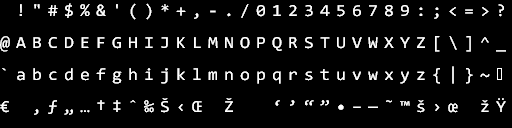
\includegraphics[width=.8\textwidth]{ExportedFont.png}
	\caption[Bitmap-Font der Schrift Consolas.]{Bitmap-Font der Schrift Consolas, erzeugt mit \enquote{Codehead's Bitmap Font Generator}~\cite{Codehead2015}.}\label{fig:bitmapfont}
\end{figure}
Um Text zu rendern, wird für jeden Buchstaben die entsprechende Stelle im Bitmap-Font ausgewählt und gezeichnet. In der Blocklib wird statt eines Bitmap-Fonts ein Rendersystem von Java, das \ac{awt}, genutzt. Damit werden zur Laufzeit mit der \ac{cpu} Texturen des gesamten zu rendernden Texts erzeugt und diese dann auf die \ac{gpu} geladen. Soll der Text angezeigt werden, kann nun die gesamte Textur gerendert werden.

Beide Methoden haben bestimmte Vor- und Nachteile. Mit Bitmap-Fonts ist die Wahl der Schriftart und -größe durch die erzeugten Texturen festgelegt, zudem ist die Geschwindigkeit des Renderings von der Menge der gerenderten Symbole abhängig. Die Methode der Blocklib hat den Vorteil, dass beliebige Fonts und Schriftgrößen genutzt werden können. Sobald eine Textur erstellt wurde, ist das Rendern des gesamten Texts sehr schnell. Probleme treten allerdings auf, wenn Text gerendert werden soll, der sich (schnell) ändert, wie beispielsweise eine Zeitanzeige oder eine Konsole, in die Text geschrieben werden kann. Jedes Mal, wenn sich der zu rendernde Text ändert, muss zuerst auf der \ac{cpu}, die anders als die \ac{gpu} nicht auf Rendering ausgelegt ist, eine neue entsprechende Textur gerendert werden. Dann muss diese auf die \ac{gpu} geladen werden, damit sie schließlich angezeigt werden kann. In den eben genannten Beispielen passiert das sehr häufig, was zu einer hohen Auslastung der \ac{cpu} und des \ac{gpu}-Busses (die Leitung, über die Daten an die \ac{gpu} geschickt werden können) führt.

Es ist möglich, die Vorteile beider Methoden zu kombinieren. Da Spiele inzwischen häufig verschiedene Schriften und Schriftgrößen nutzen, werden Bibliotheken wie FreeType~\cite{TheFreeTypeProject,Vries2020} genutzt, um zur Laufzeit Texturen von Schriften zu erzeugen, die auf die \ac{gpu} geladen und dann genutzt werden können. Dieser Ansatz kann auch in der Blocklib gewählt werden, sodass \ac{awt} nicht mehr genutzt wird, um einen bestimmten Text zu rendern, sondern um zur Laufzeit einen Bitmap-Font zu erzeugen. Zusätzlich müssen die damit verbundenen nötigen Schriftdaten, wie Breite der einzelnen Zeichen und weitere typografisch wichtige Metriken erzeugt und gespeichert werden. Alternativ wäre es möglich zwei getrennte Systeme anzubieten, ein System, das einen Bitmap-Font für sich schnell ändernde Texte nutzt, und eines, das wie bisher Texturen für lange sich selten ändernde Texte erzeugt, sodass diese gesammelt angezeigt werden können. Das zweite in der Blocklib bereits bestehende System kann auch dann weiter genutzt werden, wenn eine auf Bitmap-Fonts basierende Architektur implementiert wird.